\subsection{Генератор лексических анализаторов Lex} \label{sub116}

\textit{Lex} (в~более поздних реализациях \textit{Flex})~--- программный инструмент, который позволяет определить лексический анализатор, указывая регулярные выражения для описания шаблонов токенов. Входные обозначения для Lex обычно называют \textit{языком Lex}, а~сам инструмент~--- \textit{компилятором~Lex}. Компилятор~Lex преобразует входные шаблоны в~диаграмму переходов~\cite{Levine1992}. 

На~рис.~\ref{img:lex} показанна схема использования Lex. Входной файл \texttt{lex.l} написан на~языке Lex~и описывает генерируемый лексический анализатор. Компилятор Lex преобразует \texttt{lex.l}~в программу на~языке программирования~C в~файле с~именем \texttt{lex.yy.c}.  Этот файл компилируется компилятором~C~в файл~с названием \texttt{a.out}. Результат работы компилятора~C представляет собой работающий лексический анализатор, реализующий восходящий анализ, который может получать поток входных символов~и выдавать поток токенов~\cite{Aho2003}.

\begin{figure}[ht]
	\centering
	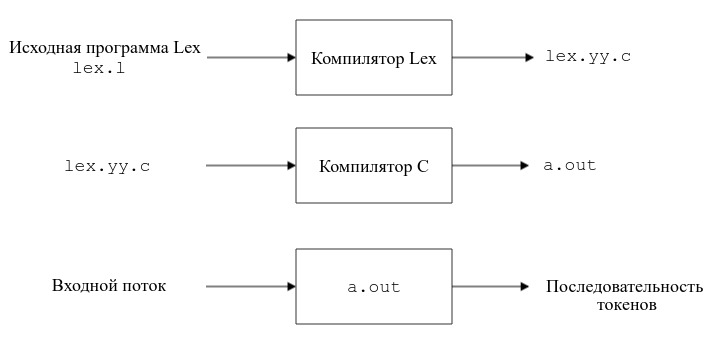
\includegraphics [scale=0.65] {lex}
	\caption{Создание лексического анализатора с~помощью Lex}
	\label{img:lex}
\end{figure}

Следующим поколением лексического генератора Lex стал Flex (fast lex). Flex практически полностью совместим с Lex. Отличия Flex:

\begin{itemize} 
	\item{может компилироваться в~C++, что позволяет использовать объектно-ориентированные конструкции~C++;}
	\item{генерирует более производительные лексические анализаторы;}
	\item{не~имеет ограничений по~размеру для таблиц символов (в~отличие от~Lex);}
	\item{небольшие синтаксические различия~\cite{Levine1992}. }
\end{itemize}
